\documentclass[10pt]{beamer}

\usepackage{isabelle,isabellesym}
\usepackage[style=authortitle,backend=bibtex]{biblatex}
\usepackage{amssymb}
\usepackage{amsmath}
\usepackage{graphicx}
\usepackage{url}
\usepackage{stmaryrd}
\usepackage{textcomp}
\usepackage[normalem]{ulem} % for striking through text 
\usepackage{fancybox}
\usepackage[all]{xypic}
\usepackage{tikz}
\usepackage{tikz-cd}
\usepackage{xcolor}
\usepackage{picture}
\usepackage{shuffle}
\usepackage{hyperref}

\hypersetup{
    colorlinks=true,
    linkcolor=cyan,
    filecolor=magenta,      
    urlcolor=blue,
    citecolor=black
}

\usetheme{default}
%\usecolortheme{seahorse}
\addbibresource{research.bib}
\setbeamertemplate{frametitle}[default][center]
\setbeamertemplate{itemize item}{$\bullet$}
\addtobeamertemplate{navigation symbols}{}{%
	\usebeamerfont{footline}%
	\usebeamercolor[fg]{footline}%
	\hspace{1em}
	\raisebox{1.6pt}[0pt][0pt]{\insertframenumber/\inserttotalframenumber}
}
\setbeamercolor{emph}{fg=white}

\usetikzlibrary{shapes,arrows,positioning,fit,backgrounds}

\graphicspath{ {./Images/} }
\isabellestyle{it}\usetikzlibrary{arrows,shapes}
\isabellestyle{it}

\newcommand{\eemph}[1]{{\color{red}#1}}
\newcommand{\mcol}[1]{\textcolor{blue}{#1}}
\newcommand{\comcol}[1]{\textcolor{violet}{#1}}

% New Commands
\newcommand{\KA}{\mathsf{KA}}
\newcommand{\MKA}{\mathsf{MKA}}
\newcommand{\KAT}{\mathsf{KAT}}
\newcommand{\rKAT}{\mathsf{rKAT}}
\newcommand{\dL}{\mathsf{d}\mathcal{L}}
\newcommand{\dH}{\mathsf{d}\mathcal{H}}
\newcommand{\dR}{\mathsf{d}\mathcal{R}}

\newcommand{\PDL}{\mathsf{PDL}}
%%%%%%%%%%%%%%%%%%%%%%%
\newcommand{\lipschitz}{\ell}
\newcommand{\norm}[1]{\left\lVert #1\right\rVert}
\newcommand{\Sup}{\mathop{Sup}}
%%%%%%%%%%%%%%%%%%%%%%%
\newcommand{\Set}{\mathbf{Set}}
\newcommand{\Rel}{\mathbf{Rel}}
\newcommand{\bools}{\mathbb{B}}
\newcommand{\nats}{\mathbb{N}}
\newcommand{\reals}{\mathbb{R}}
\newcommand{\id}{\mathit{id}}
\newcommand{\Id}{\mathit{Id}}
\newcommand{\cball}[2]{\overline{B_{#1}(#2)}}
\newcommand{\downcl}[2]{{\downarrow}\ #1\ #2}
\newcommand{\Pow}{\mathcal{P}}
%%%%%%%%%%%%%%%%%%%%%%%
\newcommand{\hoare}[3]{\{#1\}\, #2\, \{#3\}}
\newcommand{\ffbox}[2]{\mathop{|#1]}#2}
\newcommand{\ffdia}[2]{\mathop{|#1\rangle}#2}
\newcommand{\bdbox}[2]{\mathop{[#1|}#2}
\newcommand{\bddia}[2]{\mathop{\langle#1|}#2}
\newcommand{\ad}{\mathop{\mathit{ad}}}
\newcommand{\seqcomp}{\mathbin{;}}
\newcommand{\relcomp}{\seqcomp}
%%%%%%%%%%%%%%%%%%%%%%%
\newcommand{\IF}[3]{\mathbf{if}\ #1\ \mathbf{then}\ #2\ \mathbf{else}\ #3}
\newcommand{\WHILE}[2]{\mathbf{while}\ #1\ \mathbf{do}\ #2}
\newcommand{\LOOP}[1]{\mathbf{loop}\ #1}
\newcommand{\INV}[2]{#1\ \mathbf{inv}\ #2}
\newcommand{\sskip}{\mathbf{skip}}
\newcommand{\aabort}{\mathbf{abort}}
\newcommand{\wlp}{\mathit{wlp}}

\newcommand{\true}{\top}
\newcommand{\flow}{\varphi}
\newcommand{\orbit}{\gamma^\varphi}
\newcommand{\gorbit}[1]{\gamma^#1_G}
\newcommand{\WHILEI}[3]{\mathbf{while}\ #1\ \mathbf{inv}\ #2\ \mathbf{do}\ #3}
\newcommand{\Sols}{\mathop{\mathsf{Sols}}}
\newcommand{\sta}{\mathsf{Sta}}
\newcommand{\rel}{\mathsf{Rel}}
\newcommand{\inv}{\mathsf{Inv}}
%%%%%%%%%%%%%%%%%%%%%%%
\newcommand{\isactrlU}{\textbf{\textsf{U}}}
\newcommand{\unrest}{\mathop{\sharp}}
%\newcommand{\lto}{\Longrightarrow}
\newcommand{\lput}{\textit{\textsf{put}}}
\newcommand{\lget}{\textit{\textsf{get}}}
\newcommand{\lindep}{\mathop{\,\bowtie\,}}
%%%%%%%%%%%%%%%%%%%%%%%

 \newcommand{\iif}{\mathsf{if}}
 \newcommand{\ffi}{\mathsf{fi}}
 \newcommand{\tthen}{\mathsf{then}}
 \newcommand{\eelse}{\mathsf{else}}
 \newcommand{\wwhile}{\mathsf{while}}
 \newcommand{\iinv}{\mathsf{inv}}
 \newcommand{\ddo}{\mathsf{do}}
 \newcommand{\ood}{\mathsf{od}}


\everymath{\color{blue}}

 \setbeamercolor{emph}{fg=black}
 \renewcommand<>{\emph}[1]{%
   {\usebeamercolor[fg]{emph}\only#2{\itshape}#1}%
 }

\setbeamertemplate{itemize item}{$\circ$}
\setbeamertemplate{itemize subitem}{\tiny{$\triangleright$}}


 \newcommand{\rcode}[1]{\vspace{-0.5ex}
{\footnotesize
#1
}

\vspace{-3.5ex}
}

% THE IMPORTANT THING IS WHY????
% COMMUNICATE AT ADEQUATE LEVEL OF ABSTRACTION
% not too detailed as if it were a class, not too abstract as if you do not know

%%%%%%%%%%%%%%%%%%%%%%%%%%%%%%%%%%

\begin{document}

\title{Differential Hoare Logics and Refinement Calculi \\ for Hybrid Systems with Isabelle/HOL\\[.5cm]}
\author{Simon Foster$^1$\and Jonathan Juli\'an Huerta y Munive$^2$ \and Georg Struth$^2$}
%\authorrunning{Foster, Huerta y Munive and Struth}
\institute{University of York, UK \and University of Sheffield, UK}
\date{}

\begin{frame}
\titlepage
\end{frame}

%%%%%%%%%%%%%%%%%%%%%%%%%%%%%%%%%%

\begin{frame}{Verification of Hybrid Systems}
\begin{center}
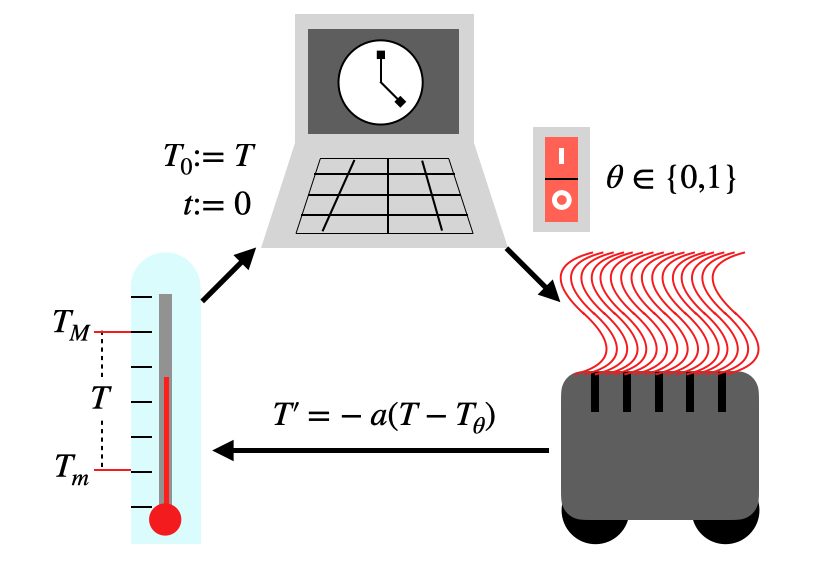
\includegraphics[scale=0.23]{thermostat.png}
\end{center}

\vspace{-.9cm}

\begin{align*}%{4}
\mathsf{dynamics}\ &=\ T'=-a(T-T_\theta)\\
\mathsf{pre}\ &=\ T_m\leq T\leq T_M\\
\mathsf{pos}\ &=\ T_m\leq T\leq T_M\\				
\mathsf{control}\ &=\ t:=0\seqcomp T_0:=T\seqcomp\dots \\
\mathsf{therm}\ &=\ (\mathsf{control}\seqcomp \mathsf{dynamics})^* &&
                 \text{\textcolor{red}{hybrid program}}\\
\mathsf{pre} &\leq\ \ffbox{\mathsf{therm}}{\mathsf{pos}} &&
                 \text{\textcolor{red}{correctness spec}}
\end{align*}
\end{frame}

%%%%%%%%%%%%%%%%%%%%%%%%%%%%%%%%%%

\begin{frame}{Previous Work}
\begin{itemize}
\item Framework for verification of hybrid programs in a general purpose proof assistant:
\begin{itemize}
\item implemented in Isabelle/HOL
\item benefits from huge, impressive libraries of topology, analysis, ODEs
\item based on $\MKA$
\item works with weakest liberal preconditions
\item supports various verification procedures for systems of ODEs
\item correct by construction
\end{itemize}
\vspace{1em}
%\item They support verification procedures for systems of ODEs:
%\begin{itemize}
%\item supply the solution;
%\item analyse invariant properties, and
%\item in the style of $\dL$.
%\end{itemize}
%\vspace{1em}
\item Yet, simpler solutions suffice for program verification:
\begin{itemize}
\item Hoare logic is enough for verification condition generation
\item Morgan's refinement calculus suffices for program construction
\end{itemize}
\end{itemize}
\vspace{\baselineskip}
\begin{center}
\comcol{Do these calculi suffice for hybrid program verification?}
\end{center}
\end{frame}

%%%%%%%%%%%%%%%%%%%%%%%%%%%%%%%%%%

\begin{frame}{Main Contributions}
Development of minimalist proof systems for hybrid system verification:
\begin{enumerate}
\item differential Hoare logic $\dH$ based on $\KAT$
\item differential refinement calculus $\dR$ based on $\rKAT$
\item integration of lenses as the store model
\item invariant reasoning in the style of differential dynamic logic $\dL$
\item tactics for automated verification condition generation
\end{enumerate}
\vspace{\baselineskip}
 \begin{center}
{\small \textcolor{blue}{\url{https://github.com/yonoteam/CPSVerification}}}
 \end{center}
\end{frame}

%%%%%%%%%%%%%%%%%%%%%%%%%%%%%%%%%%

\begin{frame}{Kleene Algebras with Tests}
\begin{block}{Kleene Algebra}
     \begin{center}
           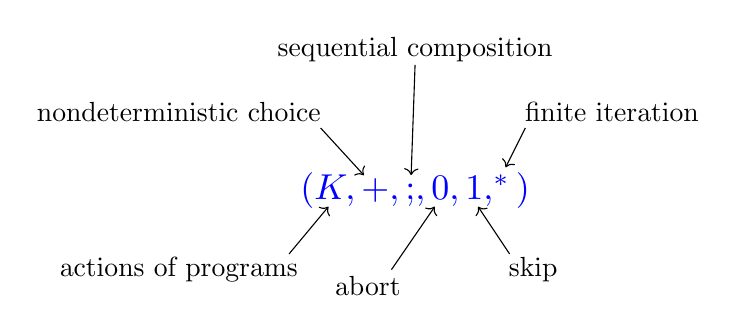
\begin{tikzpicture}
      \node at (3,1) {\scalebox{1.3}{$\mcol{(K,+,\seqcomp,0,1,^\ast)}$}};

%\uncover<2->{
\node at (0,0) {actions of programs};

\node  at (0,2) {nondeterministic choice};

\node  at (3,2.8) {sequential composition};

\node  at (5.5,2) {finite iteration};

\node  at (4.5,0) {skip};

\node at (2.4,-0.2) {abort};

\draw[->](1.4,0.2) -- (1.9,0.8);

\draw[->](1.8,1.8) -- (2.35,1.2);

\draw[->](3,2.6) -- (2.95,1.2);

\draw[->](4.4,1.8) -- (4.15,1.3);

\draw[->](2.7,0) -- (3.25,0.8);

\draw[->](4.2,0.2) -- (3.8,0.8);
%}
\end{tikzpicture}
\end{center}
\end{block}\vspace{-1.5em}
\begin{block}{Tests}
\begin{itemize}
\item $(B,+,\seqcomp,0,1,\neg)$ is a boolean algebra
\item use $\alpha,\beta\in K$ and $p,q\in B$ where $B\subseteq K$
\item $\IF{p}{\alpha}{\beta} = p\seqcomp \alpha + \neg p \seqcomp \beta$
\item $\WHILE{p}{\alpha} = (p\seqcomp \alpha)^\ast \seqcomp \neg p$
%\item $\LOOP{\alpha} = \alpha^*$, for $\alpha,\beta\in K$.
\item $\hoare{p}{\alpha}{q}\leftrightarrow p\seqcomp\alpha\leq \beta\seqcomp q$
\end{itemize}
\end{block}
\end{frame}

%%%%%%%%%%%%%%%%%%%%%%%%%%%%%%%%%%


\begin{frame}{State Transformer Model}
Programs are functions $S\to\Pow\, S$:
\begin{align*}
(\alpha + \beta)\, s = &\ \alpha\, s \cup \beta\, s\\
(\alpha \seqcomp \beta)\, s = & (\alpha\circ_K \beta)\, s = \bigcup\{\beta\, s'\mid s'\in \alpha\, s\}\\
0\, s = &\ \emptyset\\
1\, s = &\ \{s\}\\
\alpha^*\, s = &\ \bigcup_{n\geq 0}\alpha^n\, s\text{\color{black}\ where } \alpha^{0}\, s=1\, s\text{\color{black}\ and } \alpha^{n+1}=\alpha^n\circ_K\alpha\\
(\neg p)\, s = &\  
	\begin{cases}
	\{s\}, & \text{\color{black}\ if } p\, s=\emptyset\\
	\emptyset, & \text{\color{black}\  otherwise}
	\end{cases}\\
\end{align*}
\begin{center}
$\comcol{\hoare{p}{\alpha}{q}\leftrightarrow (\forall s_1.\ p\, s_1 \rightarrow (\forall s_2.\ s_2 \in \alpha\, s_1\rightarrow q\, s_2))}$
\end{center}
\end{frame}

%%%%%%%%%%%%%%%%%%%%%%%%%%%%%%%%%%

\begin{frame}{What about Assignments?}
\begin{block}{Lenses}
\begin{itemize}
\item Variables are lenses $x = (A, S, \lget_x, \lput_x)$ denoted $x : A \Longrightarrow S$ where
\begin{equation*}
\mcol{\lget_x:S\to A}\text{ and }\mcol{\lput_x:S\to A\to S}%(denoted $x : A \Longrightarrow S$)
\end{equation*}
\item $A$ is a variable type while $S$ is the source
\item They satisfy the axioms
\begin{align*}
\lget_x~(\lput_x~s~v) &= v\\ 
\lput_x~(\lput_x~s~u)~v &= \lput_x~s~v\\
\lput_x~s~(\lget_x~s) &= s
\end{align*}
%\item They allow us to model updates $f(x\mapsto e)\, s=\lput_x\, (f\, s)\, (e\, s)$ for $f:S\to S$ and $e:S\to A$.
\end{itemize}
\end{block}
%\vspace{\baselineskip}
\begin{block}{}
Semantics $S\to \Pow\, S$ for assignments is
\[\comcol{(x:=e)\, s %=\{\id(x\mapsto e)\, s\}
=\{\lput_x\, s\, (e\, s)\}}\]
\end{block}
\end{frame}

%%%%%%%%%%%%%%%%%%%%%%%%%%%%%%%%%%

\begin{frame}{Verification Rules}
\begin{itemize}
\item Traditional Hoare logic:
\begin{align*}
p_1\le p_2\land \hoare{p_2}{\alpha}{q_2}\land q_2\le q_1\ \rightarrow\ &
\hoare{p_1}{\alpha}{q_1}\\
\hoare{p}{\alpha}{r}\land\hoare{r}{\beta}{q}\rightarrow\ &\hoare{p}{\alpha\seqcomp\beta}{q}\\
\hoare{r\seqcomp p}{\alpha}{q}\land \hoare{\neg r\seqcomp p}{\beta}{q}\ \rightarrow\ &\hoare{p}{\IF{r}{\alpha}{\beta}}{q}\\
\hoare{r\seqcomp p}{\alpha}{p}\ \rightarrow\ & \hoare{p}{\WHILE{r}{\alpha}}{\neg r\seqcomp p}\\
&\hoare{\lambda s.\ q\, (\lput_x\, s\, (e\, s))}{x:=e}{q}
\end{align*}
\item Adapted to regular programs
\begin{align*}
&\hoare{p}{\sskip}{p}\\
&\hoare{p}{\aabort}{q}\\
\hoare{p}{\alpha}{q}\land\hoare{p}{\beta}{q}\rightarrow\ &\hoare{p}{\alpha+\beta}{q}\\
\hoare{p}{\alpha}{p}\rightarrow\ & \hoare{p}{\LOOP{\alpha}}{p}
\end{align*}
where $\LOOP{\alpha}=\alpha^*$, $\sskip=1$, and $\aabort=0$
\end{itemize}
\vspace{\baselineskip}
\end{frame}

%%%%%%%%%%%%%%%%%%%%%%%%%%%%%%%%%%

\begin{frame}{What about ODEs?}
\begin{block}{Vector Field}
\centering $X'\ t=f\ t\, (X\ t)$\\
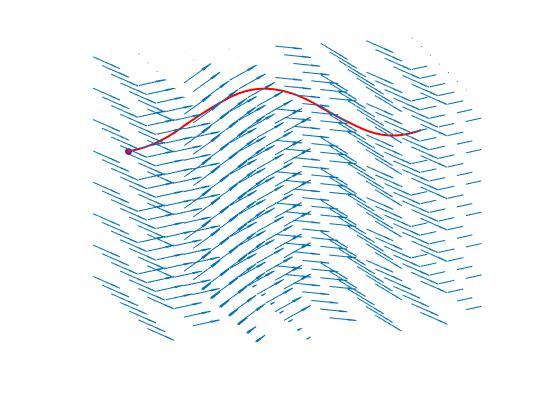
\includegraphics[width=25em,height=12.8em]{velvectors.jpg}
\end{block}\vspace{-1.5em}
where
\[\mcol{X:T\subseteq\reals\to S\qquad f:T\to S\to S\qquad X\, 0 = s}\]
\vspace{\baselineskip}
\begin{center}
$\comcol{\text{orbit}:s\mapsto \{X\, t\mid t\in T\}}$
\end{center}
\end{frame}

%%%%%%%%%%%%%%%%%%%%%%%%%%%%%%%%%%

\begin{frame}{Semantics for ODEs}

\begin{block}{}
	\begin{itemize}
	\item Solutions to initial value problems (IVPs)
\[\mcol{\Sols f\, T\, s = \left\{X:T\to S \mid (\forall t\in T.\  X'\, t = f\, t\, (X\, t)\land X\, 0 = s\right\}}\]
	\item Guarded orbit
\[\mcol{\mathsf{orbit}^X_G\, s = \{X\, t\mid t \in T\land (\forall \tau\in[0,t].\ G\, (X\, \tau))\}}\]
	\item Semantics $S\to \Pow\, S$ for assignments are
\[\mcol{(x' = f \ \&\ G)\, s = \bigcup\{\mathsf{orbit}^X_G\, s\mid X\in\Sols f\, T\, s \}}\]	
	\item The corresponding rule of inference is
\[\comcol{\{\lambda\, s.\ \forall t\in T.\ \left(\forall \tau\in [0,t].\ G\, (X\, t)\right)\to Q\, (X\, t)\}\ (x'{=}f\, \&\, G)\ \{Q\}}\]
	\end{itemize}
 \end{block}
%\vspace{\baselineskip}
\centering\comcol{easy to obtain if there is a unique solution $X:T\to S$ to the IVPs\\ associated to each $s$ and the vector field $f$}
%\begin{block}{Verification Rule}
%\begin{gather*}
%\frac{\forall s\in S.\exists!X:T\to S.\ X\, 0=s\land(\forall t\in T.\ \comcol{X'\, t=f\, t\, (X\, t)})}{\hoare{\lambda s.\ s\in S\rightarrow\forall t\in T.\ \left(\forall \tau\in [0,t].\ G\, (X\, t)\right)\to q\, (X\, t)}{x' = f \ \&\ G}{q}}
%\end{gather*}
%\end{block}
\end{frame}

%%%%%%%%%%%%%%%%%%%%%%%%%%%%%%%%%%

\begin{frame}{Invariants in $\dH$}

\begin{itemize}
\item $I$ is an invariant for $f$ iff $\hoare{I}{x'{=}f\, \&\, G}{I}$, or equivalently
\begin{equation*}
\mcol{\bigcup (\Pow\, (x'{=}f\, \&\, G)\,  I)\subseteq I}
\end{equation*}
\item We obtain the following rules
\begin{align*}
p\le i \land \hoare{i}{\alpha}{i}\land i\le q\ \rightarrow\ & \hoare{p}{\INV{\alpha}{i}}{q}\\
\hoare{i}{\alpha}{i} \land \hoare{j}{\alpha}{j}\rightarrow\ &\hoare{i\seqcomp j}{\alpha}{i\seqcomp j}\\
\hoare{i}{\alpha}{i} \land \hoare{j}{\alpha}{j}\rightarrow\ &\hoare{i+ j}{\alpha}{i+ j}\\
p \le i \land \hoare{i\seqcomp t}{\alpha}{i} \land \neg r\seqcomp i\le q\ \rightarrow \ & \hoare{p}{\INV{\WHILE{r}{\alpha}}{i}}{q}\\
p\le i \land \hoare{i}{\alpha}{i}\land i\le q\ \rightarrow\ &
\hoare{p}{\INV{\LOOP{\alpha}}{i}}{q}\\
\comcol{p\le i \land i\text{ is inv. for }f\land (G\seqcomp i)\le q\ \rightarrow}\ & \comcol{\hoare{p}{\INV{x' = f \, \&\, G}{i}}{q}}
\end{align*}
where operationally $\INV{\alpha}{i}=\alpha$
\end{itemize}
\vspace{\baselineskip}
\end{frame}

%%%%%%%%%%%%%%%%%%%%%%%%%%%%%%%%%%

\begin{frame}{Formalisation of the Thermostat}
\begin{center}
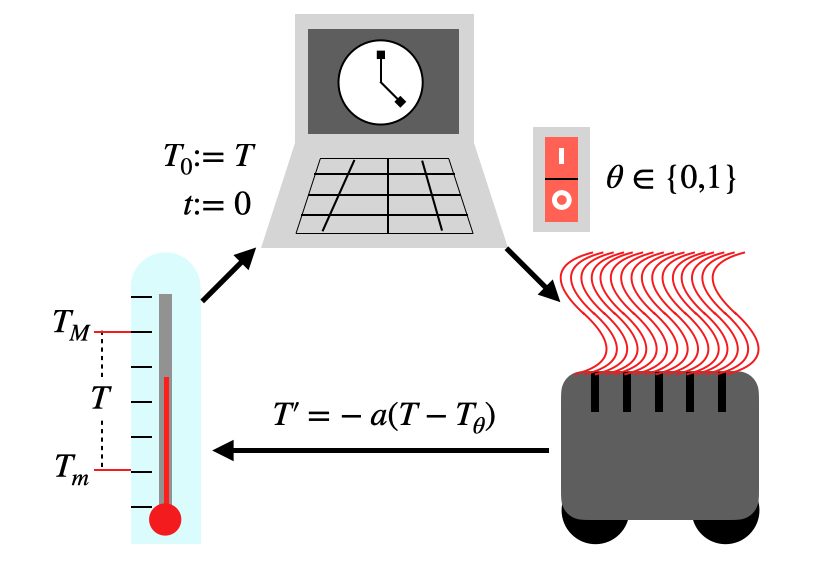
\includegraphics[scale=0.23]{thermostat.png}
\end{center}\vspace{-2em}
\alt<2->{
\begin{block}{}
Provide vector field and unique solution
\begin{isabellebody}
\isanewline
\isacommand{abbreviation}\ {\isachardoublequoteopen}\mcol{f\ a\ c\ {\isasymequiv}\ {\isacharbrackleft}T\ {\isasymmapsto}\isactrlsub s\ {\isacharminus}\ {\isacharparenleft}a\ {\isacharasterisk}\ {\isacharparenleft}T\ {\isacharminus}\ c{\isacharparenright}{\isacharparenright}{\isacharcomma}\ T\isactrlsub {\isadigit{0}}\ {\isasymmapsto}\isactrlsub s\ {\isadigit{0}}{\isacharcomma}\ {\isasymtheta}\ {\isasymmapsto}\isactrlsub s\ {\isadigit{0}}{\isacharcomma}\ t\ {\isasymmapsto}\isactrlsub s\ {\isadigit{1}}{\isacharbrackright}}{\isachardoublequoteclose}\isanewline

\isacommand{abbreviation}\ {\isachardoublequoteopen}\mcol{{\isasymphi}\ a\ c\ {\isasymtau}\ {\isasymequiv}\ {\isacharbrackleft}T\ {\isasymmapsto}\isactrlsub s\ {\isacharminus}\ $\comcol{\mathbf{exp}}$\ {\isacharparenleft}{\isacharminus}a\ {\isacharasterisk}\ {\isasymtau}{\isacharparenright}\ {\isacharasterisk}\ {\isacharparenleft}c\ {\isacharminus}\ T{\isacharparenright}\ {\isacharplus}\ c{\isacharcomma}\isanewline
\ \ \ \ T\isactrlsub {\isadigit{0}}\ {\isasymmapsto}\isactrlsub s\ T\isactrlsub {\isadigit{0}}{\isacharcomma}\ {\isasymtheta}\ {\isasymmapsto}\isactrlsub s\ {\isasymtheta}{\isacharcomma}\ t\ {\isasymmapsto}\isactrlsub s\ {\isasymtau}\ {\isacharplus}\ t{\isacharbrackright}}{\isachardoublequoteclose}\isanewline
\end{isabellebody}
\end{block}
}{
\begin{block}{}
Lenses $\Pi[n]=(\reals,\reals^{\{0,1,2,3\}},\lambda s.\ s\, n,\lambda s\, t.\ s[n\mapsto t])$ give us variables
\begin{isabellebody}
\isanewline
\isacommand{abbreviation}\isamarkupfalse%
\ \mcol{T\ {\isacharcolon}{\isacharcolon}\ {\isachardoublequoteopen}real\ {\isasymLongrightarrow}\ real{\isacharcircum}{\isadigit{4}}}{\isachardoublequoteclose}\ \isakeyword{where}\ {\isachardoublequoteopen}\mcol{T\ {\isasymequiv}\ {\isasymPi}{\isacharbrackleft}{\isadigit{0}}{\isacharbrackright}}{\isachardoublequoteclose}\isanewline
\isacommand{abbreviation}\isamarkupfalse%
\ \mcol{t\ {\isacharcolon}{\isacharcolon}\ {\isachardoublequoteopen}real\ {\isasymLongrightarrow}\ real{\isacharcircum}{\isadigit{4}}}{\isachardoublequoteclose}\ \isakeyword{where}\ {\isachardoublequoteopen}\mcol{t\ {\isasymequiv}\ {\isasymPi}{\isacharbrackleft}{\isadigit{1}}{\isacharbrackright}}{\isachardoublequoteclose}\isanewline
\isacommand{abbreviation}\isamarkupfalse%
\ \mcol{T\isactrlsub {\isadigit{0}}\ {\isacharcolon}{\isacharcolon}\ {\isachardoublequoteopen}real\ {\isasymLongrightarrow}\ real{\isacharcircum}{\isadigit{4}}}{\isachardoublequoteclose}\ \isakeyword{where}\ {\isachardoublequoteopen}\mcol{T\isactrlsub {\isadigit{0}}\ {\isasymequiv}\ {\isasymPi}{\isacharbrackleft}{\isadigit{2}}{\isacharbrackright}}{\isachardoublequoteclose}\isanewline
\isacommand{abbreviation}\isamarkupfalse%
\ \mcol{{\isasymtheta}\ {\isacharcolon}{\isacharcolon}\ {\isachardoublequoteopen}real\ {\isasymLongrightarrow}\ real{\isacharcircum}{\isadigit{4}}}{\isachardoublequoteclose}\ \isakeyword{where}\ {\isachardoublequoteopen}\mcol{{\isasymtheta}\ {\isasymequiv}\ {\isasymPi}{\isacharbrackleft}{\isadigit{3}}{\isacharbrackright}}{\isachardoublequoteclose}\isanewline
\end{isabellebody}
\end{block}}
\end{frame}

%%%%%%%%%%%%%%%%%%%%%%%%%%%%%%%%%%

\begin{frame}{Verification of the Thermostat}
\alt<2->{
\begin{center}
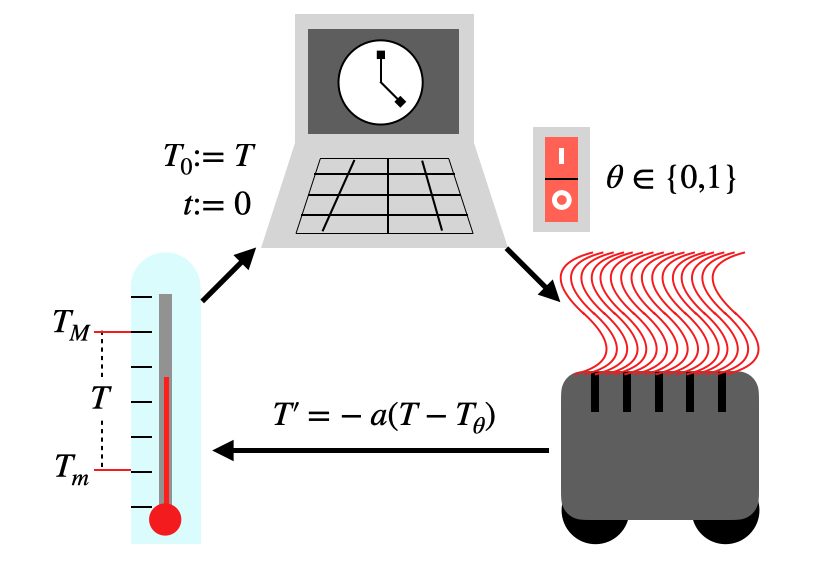
\includegraphics[scale=0.23]{thermostat.png}
\end{center}\vspace{-2em}
\begin{isabellebody}
\isanewline
\isacommand{lemma}\isamarkupfalse%
\ thermostat{\isacharunderscore}flow{\isacharcolon}\ \isanewline
\ \ \isakeyword{assumes}\ {\isachardoublequoteopen}\mcol{{\isadigit{0}}\ {\isacharless}\ a}{\isachardoublequoteclose}\ \isakeyword{and}\ {\isachardoublequoteopen}\mcol{{\isadigit{0}}\ {\isasymle}\ {\isasymtau}}{\isachardoublequoteclose}\ \isakeyword{and}\ {\isachardoublequoteopen}{\isadigit{0}}\ {\isacharless}\ $T_m${\isachardoublequoteclose}\ \isakeyword{and}\ {\isachardoublequoteopen}\mcol{$T_M$\ {\isacharless}\ $T_u$}{\isachardoublequoteclose}\isanewline
\ \ \isakeyword{shows}\ {\isachardoublequoteopen}\ \mcol{\isactrlbold {\isacharbraceleft}I\ $T_m$\ $T_M$\isactrlbold {\isacharbraceright}\ therm\ $T_m$\ $T_M$\ a\ $T_u$\ {\isasymtau}\ \isactrlbold {\isacharbraceleft}I\ $T_m$\ $T_M$\isactrlbold {\isacharbraceright}}{\isachardoublequoteclose}\isanewline
\ \ \isacommand{apply} \comcol{
{\isacharparenleft}hyb{\isacharunderscore}hoare}\ {\isachardoublequoteopen}{\isactrlU}{\isacharparenleft}\mcol{I\ $T_m$\ $T_M$\ {\isasymand}\ t{\isacharequal}{\isadigit{0}}\ {\isasymand}\ T\isactrlsub {\isadigit{0}}\ {\isacharequal}\ T{\isacharparenright}{\isachardoublequoteclose}{\isacharparenright}}\isanewline
\ \ \isacommand{prefer}\isamarkupfalse%
\ {\isadigit{4}}\ \isacommand{prefer}\isamarkupfalse%
\ {\isadigit{8}}\ \isacommand{using}\isamarkupfalse%
\ local{\isacharunderscore}flow{\isacharunderscore}therm\ assms\ \isacommand{apply}\isamarkupfalse\ force{\isacharplus}\isanewline
\ \ \isacommand{using}\isamarkupfalse%
\ assms\ therm{\isacharunderscore}dyn{\isacharunderscore}up\ therm{\isacharunderscore}dyn{\isacharunderscore}down\ \isacommand{by}\isamarkupfalse%
\ rel{\isacharunderscore}auto{\isacharprime}\isanewline
\end{isabellebody}
}{
\begin{isabellebody}
\isacommand{abbreviation}\ {\isachardoublequoteopen}\mcol{G\ $T_m$\ $T_M$\ a\ L\ {\isasymequiv}\isanewline
\ \ \isactrlU {\isacharparenleft}t\ {\isasymle}\ {\isacharminus}\ {\isacharparenleft}ln\ {\isacharparenleft}{\isacharparenleft}L{\isacharminus}{\isacharparenleft}if\ L{\isacharequal}{\isadigit{0}}\ then\ $T_m$\ else\ $T_M${\isacharparenright}{\isacharparenright}{\isacharslash}{\isacharparenleft}L{\isacharminus}T\isactrlsub {\isadigit{0}}{\isacharparenright}{\isacharparenright}{\isacharparenright}{\isacharslash}a{\isacharparenright}}{\isachardoublequoteclose}\isanewline

\isacommand{abbreviation}\ {\isachardoublequoteopen}\mcol{I\ $T_m$\ $T_M$\ {\isasymequiv}\ \isactrlU {\isacharparenleft}$T_m$\ {\isasymle}\ T\ {\isasymand}\ T\ {\isasymle}\ $T_M$\ {\isasymand}\ {\isacharparenleft}{\isasymtheta}\ {\isacharequal}\ {\isadigit{0}}\ {\isasymor}\ {\isasymtheta}\ {\isacharequal}\ {\isadigit{1}}{\isacharparenright}{\isacharparenright}}{\isachardoublequoteclose}\isanewline

\isacommand{abbreviation}\ {\isachardoublequoteopen}\mcol{ctrl\ $T_m$\ $T_M$\ {\isasymequiv}\ \isanewline
\ \ {\isacharparenleft}t\ {\isacharcolon}{\isacharcolon}{\isacharequal}\ {\isadigit{0}}{\isacharparenright}{\isacharsemicolon}\ {\isacharparenleft}T\isactrlsub {\isadigit{0}}\ {\isacharcolon}{\isacharcolon}{\isacharequal}\ T{\isacharparenright}{\isacharsemicolon}\isanewline
\ \ {\isacharparenleft}IF\ {\isacharparenleft}{\isasymtheta}\ {\isacharequal}\ {\isadigit{0}}\ {\isasymand}\ T\isactrlsub {\isadigit{0}}\ {\isasymle}\ $T_m$\ {\isacharplus}\ {\isadigit{1}}{\isacharparenright}\ THEN\ {\isacharparenleft}{\isasymtheta}\ {\isacharcolon}{\isacharcolon}{\isacharequal}\ {\isadigit{1}}{\isacharparenright}\ ELSE\ \isanewline
\ \ \ IF\ {\isacharparenleft}{\isasymtheta}\ {\isacharequal}\ {\isadigit{1}}\ {\isasymand}\ T\isactrlsub {\isadigit{0}}\ {\isasymge}\ T\isactrlsub h\ {\isacharminus}\ {\isadigit{1}}{\isacharparenright}\ THEN\ {\isacharparenleft}{\isasymtheta}\ {\isacharcolon}{\isacharcolon}{\isacharequal}\ {\isadigit{0}}{\isacharparenright}\ ELSE\ skip{\isacharparenright}}{\isachardoublequoteclose}\isanewline

\isacommand{abbreviation}\ {\isachardoublequoteopen}\mcol{dyn\ $T_m$\ $T_M$\ a\ T\isactrlsub u\ {\isasymtau}\ {\isasymequiv}\ \isanewline
\ \ IF\ {\isacharparenleft}{\isasymtheta}\ {\isacharequal}\ {\isadigit{0}}{\isacharparenright}\ THEN\ x{\isasymacute}{\isacharequal}\ f\ a\ {\isadigit{0}}\ {\isacharampersand}\ G\ $T_m$\ $T_M$\ a\ {\isadigit{0}}\ on\ {\isacharbraceleft}{\isadigit{0}}{\isachardot}{\isachardot}{\isasymtau}{\isacharbraceright}\ UNIV\ {\isacharat}\ {\isadigit{0}}\ \isanewline
\ \ \ ELSE\ x{\isasymacute}{\isacharequal}\ f\ a\ T\isactrlsub u\ {\isacharampersand}\ G\ $T_m$\ $T_M$\ a\ T\isactrlsub u\ on\ {\isacharbraceleft}{\isadigit{0}}{\isachardot}{\isachardot}{\isasymtau}{\isacharbraceright}\ UNIV\ {\isacharat}\ {\isadigit{0}}}{\isachardoublequoteclose}\isanewline

\isacommand{abbreviation}\isamarkupfalse%
\ {\isachardoublequoteopen}\mcol{therm\ $T_m$\ $T_M$\ a\ L\ {\isasymtau}\ {\isasymequiv}\isanewline
\ \ LOOP\ {\isacharparenleft}ctrl\ $T_m$\ $T_M$\ {\isacharsemicolon}\ dyn\ $T_m$\ $T_M$\ a\ L\ {\isasymtau}{\isacharparenright}\ INV\ {\isacharparenleft}I\ $T_m$\ $T_M${\isacharparenright}}{\isachardoublequoteclose}\isanewline
\end{isabellebody}
}
\end{frame}

%%%%%%%%%%%%%%%%%%%%%%%%%%%%%%%%%%

\begin{frame}{Differential Refinement Calculus $\dR$}
Extend $\KAT$ with refinement operation $[-,-]:B\times B\to K$ such that
\begin{equation*}
\mcol{\{p\}\, \alpha\, \{q\} \leftrightarrow \alpha\le [p,q]}
\end{equation*}

Obtain traditional Morgan Style Refinement laws:
\begin{align*}
\sskip &\le [p,p]\\
\aabort & \le [p,q],\\
[p',q'] &\le [p,q]\qquad \text{ if } p\le p'\text{ and } q'\le q\\
[p,r]\seqcomp [r,q] &\le [p,q]\\
[p,q]+ [p,q] &\le [p,q]\\
\IF{t}{[t\seqcomp p,q]}{[\neg t\seqcomp p,q]} &\le [p,q]\\
 \WHILE{t}{[t\seqcomp p,p]} &\le [p,\neg t\seqcomp p]\\
\LOOP{[p,p]} &\le [p,p]
\end{align*}
\end{frame}

%%%%%%%%%%%%%%%%%%%%%%%%%%%%%%%%%%

\begin{frame}{More Refinement Laws}
\begin{itemize}
\item Laws for assignments $(x := e) \le  \left[\lambda s.\ Q\, (\lput_x\, s\, (e\, s)),Q\right]$
\item Laws for evolution commands where $X'\, t = f\, (X\, t)$ and $X\, 0 = s$
\begin{gather*}
(x' = f\, \&\, G) \leq [\lambda s\in S.\forall t\in T.\ (\forall
\tau\in [0,t].\ G\, (X\, \tau))\to Q\, (X\, t),Q]%,\\
%(x' = f\, \&\, G) \seqcomp \left[Q,Q\right]\leq [\lambda s\in S. \forall t\in T.\ (\forall
%\tau\in[0,t].\ G\, (X\, \tau))\to Q\, (X\, t),Q],\\
%\left[Q,\lambda s\in S. \forall t\in T.\ (\forall
%\tau\in[0,t].\ G\, (X\, \tau))\to Q\, (X\, t)\right]\seqcomp (x' = f\, \&\, G) \leq [Q,Q].
\end{gather*}
\item Monotonoic laws and laws with invariants 
\begin{align*}
 \IF{t}{\alpha_1}{\beta_1}&\leq \IF{t}{\alpha_2}{\beta_2}\quad\text{if }\alpha_1\leq\alpha_2\text{ and }\beta_1\leq\beta_2\\
 \WHILE{t}{\alpha_1} &\leq \WHILE{t}{\alpha_2}\qquad\hspace{1.65em}\text{if }\alpha_1\leq\alpha_2\\
\LOOP{\alpha_1} &\leq \LOOP{\alpha_2}\qquad\hspace{4.3em}\text{if }\alpha_1\leq\alpha_2\\
\INV{\WHILE{t}{\alpha}}{i}&\leq [p,q]\quad\text{if }
p \le i\seqcomp t\text{ and }\alpha\leq[i,i]\text{ and }\neg t\seqcomp i\le q\\
\INV{\LOOP{\alpha}}{i}&\leq[p,q]\quad\text{if }
p \le i\text{ and }\alpha\leq[i,i]\text{ and } i\le q
\end{align*}
\end{itemize}
\vspace{\baselineskip}
\end{frame}

%%%%%%%%%%%%%%%%%%%%%%%%%%%%%%%%%%

\begin{frame}{Conclusions}
\begin{itemize}
\item Used modular semantic framework in Isabelle/HOL to
	\begin{itemize}
	\item derive a minimalist logic $\dH$ for verification of hybrid programs
	\item obtain refinement components via the laws of $\dR$
	\end{itemize}
\item Lenses provide
	\begin{itemize}
	\item a more algebraic program store
	\item better parsing: nicer syntax
	\end{itemize}
\item Future work:
	\begin{itemize}
	\item Explore total correctness
	\item Adversarial dynamics and other extensions of $\dL$
	\item Extension of related libraries of formalised mathematics 
	\item Code generation for verified executable code
	\item Integrate with a CAS that supplies solutions and invariants, leaving the certification work to Isabelle
	\end{itemize}
\end{itemize}
\vspace{\baselineskip}
\begin{center}
{\small \textcolor{blue}{\url{https://github.com/yonoteam/CPSVerification}}}
\end{center}
\end{frame}

%%%%%%%%%%%%%%%%%%%%%%%%%%%%%%%%%%

\begin{frame}{Refinement of the Thermostat}
\alt<2->{
\begin{isabellebody}
\isacommand{abbreviation}\ {\isachardoublequoteopen}\mcol{ctrl\ $T_m$\ $T_M$\ {\isasymequiv}\ \isanewline
\ \ {\isacharparenleft}t\ {\isacharcolon}{\isacharcolon}{\isacharequal}\ {\isadigit{0}}{\isacharparenright}{\isacharsemicolon}\ {\isacharparenleft}T\isactrlsub {\isadigit{0}}\ {\isacharcolon}{\isacharcolon}{\isacharequal}\ T{\isacharparenright}{\isacharsemicolon}\isanewline
\ \ {\isacharparenleft}IF\ {\isacharparenleft}{\isasymtheta}\ {\isacharequal}\ {\isadigit{0}}\ {\isasymand}\ T\isactrlsub {\isadigit{0}}\ {\isasymle}\ $T_m$\ {\isacharplus}\ {\isadigit{1}}{\isacharparenright}\ THEN\ {\isacharparenleft}{\isasymtheta}\ {\isacharcolon}{\isacharcolon}{\isacharequal}\ {\isadigit{1}}{\isacharparenright}\ ELSE\ \isanewline
\ \ \ IF\ {\isacharparenleft}{\isasymtheta}\ {\isacharequal}\ {\isadigit{1}}\ {\isasymand}\ T\isactrlsub {\isadigit{0}}\ {\isasymge}\ T\isactrlsub h\ {\isacharminus}\ {\isadigit{1}}{\isacharparenright}\ THEN\ {\isacharparenleft}{\isasymtheta}\ {\isacharcolon}{\isacharcolon}{\isacharequal}\ {\isadigit{0}}{\isacharparenright}\ ELSE\ skip{\isacharparenright}}{\isachardoublequoteclose}\isanewline

\isacommand{lemma}\ R{\isacharunderscore}therm{\isacharunderscore}time{\isacharcolon}\ {\isachardoublequoteopen}\mcol{\isactrlbold {\isacharbrackleft}I\ $T_m$\ $T_M${\isacharcomma}\ I\ $T_m$\ $T_M$\ {\isasymand}\ t\ {\isacharequal}\ {\isadigit{0}}\isactrlbold {\isacharbrackright}\ {\isasymge}\ {\isacharparenleft}t\ {\isacharcolon}{\isacharcolon}{\isacharequal}\ {\isadigit{0}}{\isacharparenright}}{\isachardoublequoteclose}\isanewline
\ \ \isacommand{by}\isamarkupfalse%
\ {\isacharparenleft}rule\ R{\isacharunderscore}assign{\isacharunderscore}law{\isacharcomma}\ pred{\isacharunderscore}simp{\isacharparenright}\isanewline

\isacommand{lemma}\ R{\isacharunderscore}therm{\isacharunderscore }temp{\isacharcolon}\isanewline 
\ \ {\isachardoublequoteopen}\mcol{\isactrlbold {\isacharbrackleft}I\ $T_m$\ $T_M$\ {\isasymand}\ t\ {\isacharequal}\ {\isadigit{0}}{\isacharcomma}\ I\ $T_m$\ $T_M$\ {\isasymand}\ t\ {\isacharequal}\ {\isadigit{0}}\ {\isasymand}\ T\isactrlsub {\isadigit{0}}\ {\isacharequal}\ T\isactrlbold {\isacharbrackright}\ {\isasymge}\ {\isacharparenleft}T\isactrlsub {\isadigit{0}}\ {\isacharcolon}{\isacharcolon}{\isacharequal}\ T{\isacharparenright}}{\isachardoublequoteclose}\isanewline
\ \ \isacommand{by}\isamarkupfalse%
\ {\isacharparenleft}rule\ R{\isacharunderscore}assign{\isacharunderscore}law{\isacharcomma}\ pred{\isacharunderscore}simp{\isacharparenright}\isanewline

\isacommand{lemma}\ R{\isacharunderscore}thermostat{\isacharunderscore }flow{\isacharcolon}\isanewline
\ \ \isakeyword{assumes}\ {\isachardoublequoteopen}\mcol{a\ {\isachargreater}\ {\isadigit{0}}}{\isachardoublequoteclose}\ \isakeyword{and}\ {\isachardoublequoteopen}\mcol{{\isadigit{0}}\ {\isasymle}\ {\isasymtau}}{\isachardoublequoteclose}\ \isakeyword{and}\ {\isachardoublequoteopen}\mcol{{\isadigit{0}}\ {\isacharless}\ $T_m$}{\isachardoublequoteclose}\ \isakeyword{and}\ {\isachardoublequoteopen}\mcol{$T_M$\ {\isacharless}\ T\isactrlsub u}{\isachardoublequoteclose}\isanewline
\ \ \isakeyword{shows}\ {\isachardoublequoteopen}\mcol{\isactrlbold {\isacharbrackleft}I\ $T_m$\ $T_M${\isacharcomma}\ I\ $T_m$\ $T_M$\isactrlbold {\isacharbrackright}\ {\isasymge}\ therm\ $T_m$\ $T_M$\ a\ T\isactrlsub u\ {\isasymtau}}{\isachardoublequoteclose}\isanewline
\ \ \isacommand{by}\isamarkupfalse%
\ {\isacharparenleft}refinement{\isacharsemicolon}{\isacharparenleft}rule\ R{\isacharunderscore}therm{\isacharunderscore}time{\isacharparenright}{\isacharquery}{\isacharcomma}{\isacharparenleft}rule\ R{\isacharunderscore}therm{\isacharunderscore}temp{\isacharparenright}{\isacharquery}{\isacharcomma}\isanewline
\ \ \ \ \ {\isacharparenleft}rule\ R{\isacharunderscore }assign{\isacharunderscore}law{\isacharparenright}{\isacharquery}{\isacharcomma}\ {\isacharparenleft}rule\ R{\isacharunderscore}therm{\isacharunderscore}up{\isacharbrackleft}OF\ assms{\isacharbrackright}{\isacharparenright}{\isacharquery}{\isacharcomma}\isanewline
\ \ \ \ \ \ {\isacharparenleft}rule\ R{\isacharunderscore }therm{\isacharunderscore}down{\isacharbrackleft}OF\ assms{\isacharbrackright}{\isacharparenright}{\isacharquery}{\isacharparenright}\ rel{\isacharunderscore}auto{\isacharprime}
\isanewline
\end{isabellebody}
}{
\begin{isabellebody}
\isacommand{abbreviation}\ {\isachardoublequoteopen}\mcol{dyn\ $T_m$\ $T_M$\ a\ T\isactrlsub u\ {\isasymtau}\ {\isasymequiv}\ \isanewline
\ \ IF\ {\isacharparenleft}{\isasymtheta}\ {\isacharequal}\ {\isadigit{0}}{\isacharparenright}\ THEN\ x{\isasymacute}{\isacharequal}\ f\ a\ {\isadigit{0}}\ {\isacharampersand}\ G\ $T_m$\ $T_M$\ a\ {\isadigit{0}}\ on\ {\isacharbraceleft}{\isadigit{0}}{\isachardot}{\isachardot}{\isasymtau}{\isacharbraceright}\ UNIV\ {\isacharat}\ {\isadigit{0}}\ \isanewline
\ \ \ ELSE\ x{\isasymacute}{\isacharequal}\ f\ a\ T\isactrlsub u\ {\isacharampersand}\ G\ $T_m$\ $T_M$\ a\ T\isactrlsub u\ on\ {\isacharbraceleft}{\isadigit{0}}{\isachardot}{\isachardot}{\isasymtau}{\isacharbraceright}\ UNIV\ {\isacharat}\ {\isadigit{0}}}{\isachardoublequoteclose}\isanewline

\isacommand{lemma}\isamarkupfalse%
\ R{\isacharunderscore}therm{\isacharunderscore}down{\isacharcolon}\ \isanewline
\ \ \isakeyword{assumes}\ {\isachardoublequoteopen}\mcol{a\ {\isachargreater}\ {\isadigit{0}}}{\isachardoublequoteclose}\ \isakeyword{and}\ {\isachardoublequoteopen}\mcol{{\isadigit{0}}\ {\isasymle}\ {\isasymtau}}{\isachardoublequoteclose}\ \isakeyword{and}\ {\isachardoublequoteopen}\mcol{{\isadigit{0}}\ {\isacharless}\ $T_m$}{\isachardoublequoteclose}\ \isakeyword{and}\ {\isachardoublequoteopen}\mcol{$T_M$\ {\isacharless}\ T\isactrlsub u}{\isachardoublequoteclose}\isanewline
\ \ \isakeyword{shows}\ {\isachardoublequoteopen}\mcol{\isactrlbold {\isacharbrackleft}{\isasymtheta}\ {\isacharequal}\ {\isadigit{0}}\ {\isasymand}\ I\ $T_m$\ $T_M$\ {\isasymand}\ t\ {\isacharequal}\ {\isadigit{0}}\ {\isasymand}\ T\isactrlsub {\isadigit{0}}\ {\isacharequal}\ T{\isacharcomma}\ I\ $T_m$\ $T_M$\isactrlbold {\isacharbrackright}\ {\isasymge}\isanewline 
\ \ {\isacharparenleft}x{\isasymacute}{\isacharequal}\ f\ a\ {\isadigit{0}}\ {\isacharampersand}\ G\ $T_m$\ $T_M$\ a\ {\isadigit{0}}\ on\ {\isacharbraceleft}{\isadigit{0}}{\isachardot}{\isachardot}{\isasymtau}{\isacharbraceright}\ UNIV\ {\isacharat}\ {\isadigit{0}}{\isacharparenright}}{\isachardoublequoteclose}\isanewline
\ \ \isacommand{apply}{\color{black}{\isacharparenleft}rule\ local{\isacharunderscore}flow{\isachardot}R{\isacharunderscore }g{\isacharunderscore}ode{\isacharunderscore}ivl{\isacharbrackleft}OF\ local{\isacharunderscore}flow{\isacharunderscore}therm{\isacharbrackright}{\isacharparenright}}\isanewline
\ \ \isacommand{using}\isamarkupfalse%
\ therm{\isacharunderscore}dyn{\isacharunderscore }down{\isacharbrackleft}OF\ assms{\isacharparenleft}{\isadigit{1}}{\isacharcomma}{\isadigit{3}}{\isacharparenright}{\isacharcomma}\ of\ {\isacharunderscore}\ $T_M${\isacharbrackright}\ assms\ \isacommand{by}\isamarkupfalse%
\ rel{\isacharunderscore}auto{\isacharprime}\isanewline

\isacommand{lemma}\isamarkupfalse%
\ R{\isacharunderscore}therm{\isacharunderscore}up{\isacharcolon}\ \isanewline
\ \ \isakeyword{assumes}\ {\isachardoublequoteopen}\mcol{a\ {\isachargreater}\ {\isadigit{0}}}{\isachardoublequoteclose}\ \isakeyword{and}\ {\isachardoublequoteopen}\mcol{{\isadigit{0}}\ {\isasymle}\ {\isasymtau}}{\isachardoublequoteclose}\ \isakeyword{and}\ {\isachardoublequoteopen}\mcol{{\isadigit{0}}\ {\isacharless}\ $T_m$}{\isachardoublequoteclose}\ \isakeyword{and}\ {\isachardoublequoteopen}\mcol{$T_M$\ {\isacharless}\ T\isactrlsub u}{\isachardoublequoteclose}\isanewline
\ \ \isakeyword{shows}\ {\isachardoublequoteopen}\mcol{\isactrlbold {\isacharbrackleft}{\isasymnot}\ {\isasymtheta}\ {\isacharequal}\ {\isadigit{0}}\ {\isasymand}\ I\ $T_m$\ $T_M$\ {\isasymand}\ t\ {\isacharequal}\ {\isadigit{0}}\ {\isasymand}\ T\isactrlsub {\isadigit{0}}\ {\isacharequal}\ T{\isacharcomma}\ I\ $T_m$\ $T_M$\isactrlbold {\isacharbrackright}\ {\isasymge}\isanewline
\ \ {\isacharparenleft}x{\isasymacute}{\isacharequal}\ f\ a\ T\isactrlsub u\ {\isacharampersand}\ G\ $T_m$\ $T_M$\ a\ T\isactrlsub u\ on\ {\isacharbraceleft}{\isadigit{0}}{\isachardot}{\isachardot}{\isasymtau}{\isacharbraceright}\ UNIV\ {\isacharat}\ {\isadigit{0}}{\isacharparenright}}{\isachardoublequoteclose}\isanewline
\ \ \isacommand{apply}\isamarkupfalse%
{\isacharparenleft}rule\ local{\isacharunderscore}flow{\isachardot}R{\isacharunderscore }g{\isacharunderscore}ode{\isacharunderscore}ivl{\isacharbrackleft}OF\ local{\isacharunderscore}flow{\isacharunderscore}therm{\isacharbrackright}{\isacharparenright}\isanewline
\ \ \isacommand{using}\isamarkupfalse%
\ therm{\isacharunderscore}dyn{\isacharunderscore}up{\isacharbrackleft}OF\ assms{\isacharparenleft}{\isadigit{1}}{\isacharparenright}\ {\isacharunderscore}\ {\isacharunderscore}\ assms{\isacharparenleft}{\isadigit{4}}{\isacharparenright}{\isacharcomma}\ of\ $T_m${\isacharbrackright}\ assms\ \isacommand{by}\isamarkupfalse%
\ rel{\isacharunderscore}auto{\isacharprime}%
\end{isabellebody}
}
\end{frame}

%%%%%%%%%%%%%%%%%%%%%%%%%%%%%%%%%%

\begin{frame}{Verification Rules of $\dH$}
\begin{block}{\mbox{}}
\begin{gather*}
\frac{}{\hoare{q}{1}{q}}\qquad
\frac{}{\hoare{\lambda s.\ q\, (\lput_x\, s\, (e\, s))}{x:=e}{q}}\qquad
\frac{\hoare{p}{\alpha}{r}\quad\hoare{r}{\beta}{q}}{\hoare{p}{\alpha;\beta}{q}}\\
\mbox{}\\
\mbox{}\\
\frac{\hoare{r\land p}{\alpha}{q}\quad\hoare{\neg r\land p}{\beta}{q}}{\hoare{p}{\IF{r}{\alpha}{\beta}}{q}}\qquad
\frac{\hoare{p\land r}{\alpha}{q}}{\hoare{p}{\WHILE{r}{\alpha}}{\neg r\land q}}\\
\mbox{}\\
\mbox{}\\
\frac{p\to r_1\quad\hoare{r_1}{\alpha}{r_2}\quad r_2\to q}{\hoare{p}{\alpha}{q}}
\mbox{}\\
\mbox{}\\
\comcol{\frac{\forall s\in S.\exists!X:T\to S.\ X\, 0=s\land(\forall t\in T.\ X'\, t=f\, t\, (X\, t))}{\hoare{\lambda s.\ s\in S\rightarrow\forall t\in T.\ \left(\forall \tau\in [0,t].\ G\, (X\, t)\right)\to q\, (X\, t)}{x' = f \ \&\ G}{q}}}
\end{gather*}
\end{block}
\vspace{\baselineskip}
\end{frame}

%%%%%%%%%%%%%%%%%%%%%%%%%%%%%%%%%%

\begin{frame}{Extended verification Rules of $\dH$}
\begin{block}{\mbox{}}
\begin{gather*}
\frac{}{\hoare{q}{1}{q}}\qquad
\frac{}{\hoare{\lambda s.\ q\, (\lput_x\, s\, (e\, s))}{x:=e}{q}}\qquad
\frac{}{\hoare{p}{0}{q}}\qquad\\
\mbox{}\\
\mbox{}\\
\frac{\hoare{p}{\alpha}{q}\quad\hoare{p}{\beta}{q}}{\hoare{p}{\alpha+\beta}{q}}\qquad
\frac{\hoare{p}{\alpha}{r}\quad\hoare{r}{\beta}{q}}{\hoare{p}{\alpha;\beta}{q}}\\
\mbox{}\\
\mbox{}\\
\frac{p\to r_1\quad\hoare{r_1}{\alpha}{r_2}\quad r_2\to q}{\hoare{p}{\alpha}{q}}\qquad
\frac{\hoare{p}{\alpha}{p}}{\hoare{p}{\alpha^*}{p}}
\mbox{}\\
\mbox{}\\
\comcol{\frac{\forall s\in S.\exists!X:T\to S.\ X\, 0=s\land(\forall t\in T.\ X'\, t=f\, t\, (X\, t))}{\hoare{\lambda s.\ s\in S\rightarrow\forall t\in T.\ \left(\forall \tau\in [0,t].\ G\, (X\, t)\right)\to q\, (X\, t)}{x' = f \ \&\ G}{q}}}
\end{gather*}
\end{block}
\vspace{\baselineskip}
\end{frame}


\end{document}